% !TeX program = pdflatex
% !TeX encoding = UTF-8
% !TeX spellcheck = en_GB

\documentclass[9pt, handout]{beamer}

%********************************************************************
% Packages
%********************************************************************

\usepackage[utf8]{inputenc}
\usepackage[T1]{fontenc}
\usepackage[english]{babel}
\usepackage[bottom, para]{footmisc}
\usepackage{amsmath,amssymb,amsthm}
\usepackage{graphicx}
\usepackage{hyperref}
\usepackage{listings}
\usepackage{perpage}
\usepackage{xcolor}
\usepackage{wrapfig}
\usepackage{ifthen}
\usepackage{scrextend} % add margin to answers
\usepackage{dashrule}

%********************************************************************
% Packages options
%********************************************************************

% geometry
\usepackage{geometry}
\geometry{
    a4paper,
    ignoremp,
    bindingoffset = 1cm, 
    textwidth     = 13.5cm,
    textheight    = 21.5cm,
    lmargin       = 1cm,
    rmargin		    = 3cm,
    tmargin       = 2cm,
    bmargin       = 3cm
}

% listings
\renewcommand{\lstlistingname}{Code}

\definecolor{lightgray}{rgb}{.9,.9,.9}
\definecolor{darkgray}{rgb}{.4,.4,.4}
\definecolor{purple}{rgb}{0.65, 0.12, 0.82}
\lstset{
  basicstyle=\small\sffamily,
  numbers=left,
  numberstyle=\tiny,
  numbersep=3pt,
  stepnumber=1,
  frame=tb,
  columns=fullflexible,
  backgroundcolor=\color{yellow!15},
  keywordstyle=\color{blue}\bfseries,
  ndkeywordstyle=\color{darkgray}\bfseries,
  identifierstyle=\color{black},
  commentstyle=\color{purple}\ttfamily,
  stringstyle=\color{red}\ttfamily,
  numberbychapter=false,
  showstringspaces=false,
  breaklines=true,
  captionpos=b, % put captions at the bottom 
}
%\lstset{
%  numbersep=5pt,
%  frame=trbl
%}

\definecolor{prismgreen}{rgb}{0.12, 0.48, 0.12}
\lstdefinelanguage{prism}{ % syntax highlight via font
  keywords={
    bool,C,ceil,const,ctmc,double,dtmc,endinit,endmodule,endrewards,endsystem,F,false,floor,formula,G,global,I,init,int,label,max,mdp,min,module,nondeterministic,P,Pmin,Pmax,prob,probabilistic,R,rate,rewards,Rmin,Rmax,S,stochastic,system,true,U,X
  }, 
  keywordstyle={\bfseries\color{black}}, 
  numberstyle=\tiny\color{black}, 
  comment=[l] {//}, morecomment=[s]{/*}{*/}, % single and multi-line 
  commentstyle= \color{prismgreen}, % dark green 
  tabsize=4, % tab treatment (going to be fixed in Prism)
  escapechar=@ % write LaTeX comments escaped by @ symbol 
} 

% perpage
\MakePerPage{footnote}

% hyperref
\definecolor{webgreen}{rgb}{0,.5,0}
\definecolor{webbrown}{rgb}{.6,0,0}
\definecolor{RoyalBlue}{cmyk}{1, 0.50, 0, 0}
\hypersetup{%
  %draft, % = no hyperlinking at all (useful in b/w printouts)
  colorlinks=true, linktocpage=true, pdfstartpage=3, pdfstartview=FitV,%
  % uncomment the following line if you want to have black links (e.g., for printing)
  % colorlinks=false, linktocpage=false, pdfstartpage=3, pdfstartview=FitV, pdfborder={0 0 0},%
  breaklinks=true, pdfpagemode=UseNone, pageanchor=true, pdfpagemode=UseOutlines,%
  plainpages=false, bookmarksnumbered, bookmarksopen=true, bookmarksopenlevel=1,%
  hypertexnames=true, pdfhighlight=/O,%nesting=true,%frenchlinks,%
  urlcolor=RoyalBlue, linkcolor=black, citecolor=webbrown, %pagecolor=RoyalBlue,%
  %urlcolor=Black, linkcolor=Black, citecolor=Black, %pagecolor=Black,%
}

% graphicx
\graphicspath{{img/}}

%********************************************************************
% New commands
%********************************************************************

\newcommand{\question}[1]{%
  \vspace{20pt}%
  \begin{wrapfigure}{l}{0.1\textwidth}%
    \vspace{-30pt}%
    \begin{center}%
      
\includegraphics[scale=1]{hand.jpg}%
    \end{center}%
    \vspace{-30pt}%
  \end{wrapfigure}%
  \noindent #1%
}%
\newcommand{\answer}[1]{%
  \vspace{5pt}\par\noindent
  \textbf{\underline{Answer:}}%
  \begin{addmargin}[1em]{1em}% 1em left, 2em right
    #1%
    \begin{flushright}%
      \qedsymbol%
    \end{flushright}%
  \end{addmargin}%
}%

\definecolor{light-gray}{gray}{0.95}
\newboolean{inlineCodeBackground}
\setboolean{inlineCodeBackground}{false}
\newcommand{\prism}[1]{%
  \ifthenelse{\boolean{inlineCodeBackground}}{%
    \colorbox{light-gray}{\lstinline[language=prism]{#1}}%
  }{%
    \lstinline[language=prism]{#1}%
  }%
}%
\newcommand{\bash}[1]{%
  \ifthenelse{\boolean{inlineCodeBackground}}{%
    \colorbox{light-gray}{\lstinline[language=bash]{#1}}%
  }{%
    \lstinline[language=bash]{#1}%
  }%
}%

\newcommand{\dashedrule}{%
  \noindent\hdashrule{\textwidth}{1pt}{1.5mm}%
}%


\title[AAL: Fuzzy Logic \& Stochastic Modelling]{
  Ambient Assisted Living:\\
  Fuzzy Logic \& Stochastic Modelling
}
\author{\textbf{Tommaso Papini}}
\institute{
  STLab, Department of Information Engineering, University of Florence, Italy,\\
  {tommaso.papini@unifi.it}
}
\date{
  29th June 2017
}

\begin{document}

  \begin{frame}
    \titlepage
    \begin{itemize}
      \item Ambient Assisted Living
      \item Activity Recognition
      \begin{itemize}
        \item A Fuzzy Logic approach
        \item A Stochastic Model approach
      \end{itemize}
      \item A joint proposal
    \end{itemize}
  \end{frame}

  \begin{frame}{Overview}
    %\tiny
    \tableofcontents
  \end{frame}
  
  \section{Ambient Assisted Living}
    
    \begin{frame}{Ambient Assisted Living}
      \textbf{Ambient Assisted Living} is a research area that aims to help those people living within \textit{smart environments} (i.e., provided with sensors and actuators) exploiting sensors and data processing technology.
      
      \begin{center}
        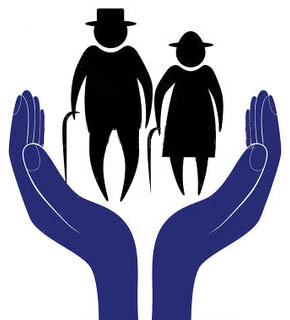
\includegraphics[scale=1.8]{elderly_assi.jpg}
      \end{center}
    \end{frame}
    
    \subsection{Problem description}
      \begin{frame}{Objectives}
        \pause
        A \textit{smart environment} is a \textbf{partially observable} system:
        \pause
        \begin{itemize}
          \item the actual state of the system is hidden;
          \pause
          \item only events are observables (\textit{observations}) as they are emitted by the system (e.g. the activation of a sensor).
        \end{itemize}
        
        \vspace{1em}
        \pause
        Main analyses of interest:
        \pause
        \begin{itemize}
          \item \textbf{Diagnosis}: (a.k.a. Activity Recognition, AR) esteem the actual present state of the system from the events observed.
          \pause
          \item \textbf{Prediction}: esteem what's going to be the actual system's state after a certain amount of time or the probability density function that a certain event happens.
          \pause
          \item \textbf{Action scheduling}: chose the best action and when to execute it in order to avoid critical situations.
        \end{itemize}
        
        \vspace{1em}
        \pause
        Online analysis:
        \pause
        \begin{itemize}
          \item analyse the system \textit{while} it is evolving.
        \end{itemize}
      \end{frame}
      
      \begin{frame}{Activity Recognition}
        \pause
        Activity Recognition techniques can be divided into two classes:
        \pause
        \begin{itemize}
          \item \textbf{Knowledge-Driven Approaches} (KDA)
          \begin{itemize}
            \item domain-specific expert knowledge is used in order to build the AR model.
          \end{itemize}
          \pause
          \item \textbf{Data-Driven Approaches} (DDA)
          \begin{itemize}
            \item a training dataset is used in order to automatically build the AR model, in a supervised fashion.
          \end{itemize}
        \end{itemize}
        
        \pause
        Comparative survey between AR researches:
        \pause
        \begin{itemize}
          \item \textit{STLab} research group\footnote{\url{https://stlab.dinfo.unifi.it/}}
          \begin{itemize}
            \item stochastic modelling techniques.
          \end{itemize}
          \pause
          \item \textit{Sinbad\textsuperscript{2}} research group\footnote{\url{http://sinbad2.ujaen.es/}}
          \begin{itemize}
            \item fuzzy logic techniques and temporal window-based classification
          \end{itemize}
        \end{itemize}
      \end{frame}
      
    \subsection{Annotated datasets}
      \begin{frame}{Annotated datasets}
        \pause
        An  \textit{annotated dataset} of a partially observable system is a dataset with:
        \pause
        \begin{itemize}
          \item recorded events and when each happened (timestamp);
          \pause
          \item manual annotations of the evolution of the actual state of the system (with time intervals for each state).
        \end{itemize}
        
        \pause
        \vspace{1em}
        \visible<5->{
          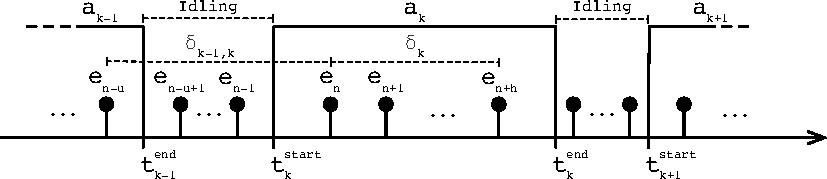
\includegraphics[scale=0.8]{activity_event_formulation.pdf}
        }
      \end{frame}
      
      \begin{frame}{Annotated datasets}{van Kasteren}
        A classic example is the \textit{van Kasteren}\footnote{\url{https://sites.google.com/site/tim0306/datasets}}\footnote{Van Kasteren, T., Noulas, A., Englebienne, G. and Kröse, B., 2008, September. Accurate activity recognition in a home setting. In Proceedings of the 10th international conference on Ubiquitous computing (pp. 1-9). ACM.} annotated dataset for AAL
        
        \pause
        \visible<2->{
          \begin{center}
            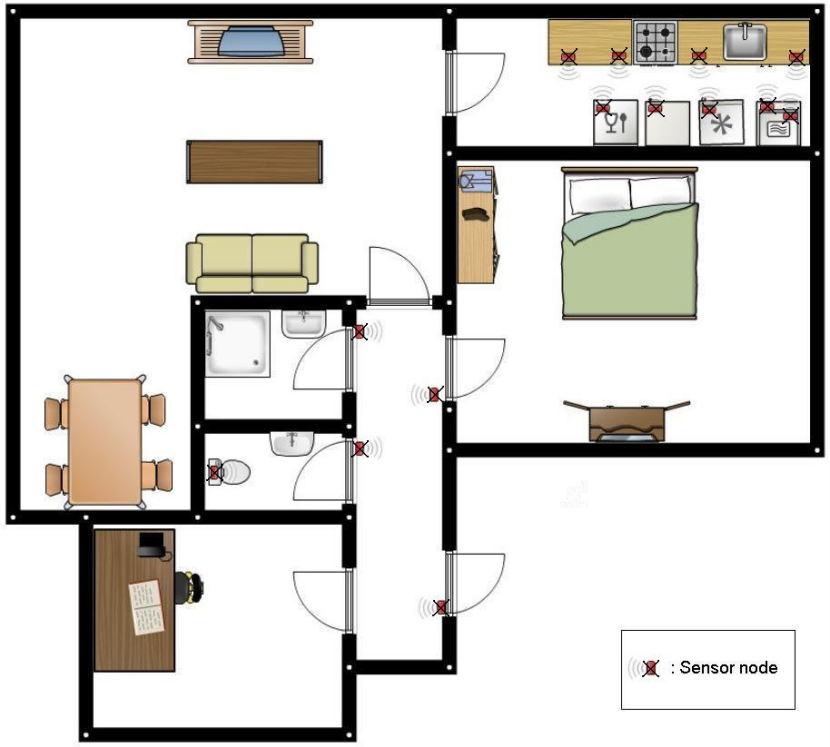
\includegraphics[scale=0.18]{SmartHome.png}
          \end{center}
        }
      \end{frame}
      
      \begin{frame}{Annotated datasets}{van Kasteren}
        \pause
        \begin{itemize}
          \item 7+1 types of activities (Activities of Daily Living, ADL\footnote{Katz, S., Downs, T.D., Cash, H.R. and Grotz, R.C., 1970. Progress in development of the index of ADL. The gerontologist, 10(1 Part 1), pp.20-30.}):
          \begin{itemize}
            \item \{Leaving house, Preparing a beverage, Preparing breakfast, Preparing dinner, Sleeping, Taking shower, Toileting\} $\cup$ \{Idling\}.
          \end{itemize}
          \pause
          \item 28 types of events (on/off of 14 sensors):
          \begin{itemize}
            \item toilet door open/closed, fridge open/closed, \dots.
          \end{itemize}
          \pause
          \item 28 of events and annotated activities:
          \begin{itemize}
            \item 245 activities, annotated through a Bluetooth device with voice recognition;
            \item 219 \textit{Idling} intervals;
            \item 2638 observed events.
          \end{itemize}
        \end{itemize}
      \end{frame}
      
  \section{A Fuzzy Logic approach}
    \begin{frame}{A Fuzzy Logic approach}
      \pause
      A Knowledge-Driven Approach for Activity Recognition:\footnote{Medina, J., Espinilla, M., Moya, F., and Nugent, C. Activity recognition by means of rule-based inference engine based on fuzzy linguistic approach. In 13th Scandinavian Conference on Artificial Intelligence Halmstad (November 2015 2015).}
      \pause
      \begin{itemize}
        \item expert knowledge to define \textbf{time} and \textbf{sensor-specific fuzzy sets};
        \pause
        \item expert knowledge to define \textbf{classification fuzzy rules}.
      \end{itemize}
      
      \pause
      \visible<5->{
        \begin{center}
          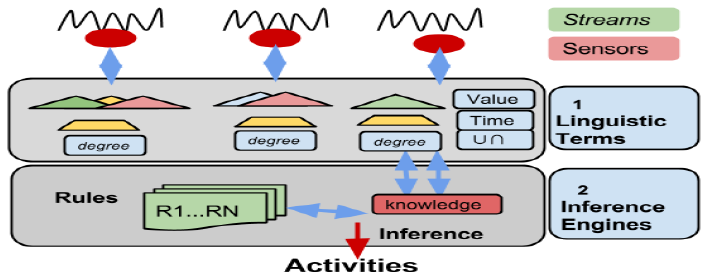
\includegraphics[scale=0.8]{fuzzy-phases.png}
        \end{center}
      }
    \end{frame}
    
    \begin{frame}{Definitions}
      \pause
      \begin{itemize}
        \item Each sensor $j$ has an associated sensor stream $s^j$;
        \pause
        \item sensor stream $s^j = \{m^j_i\}$ set of measures;
        \pause
        \item measure $m^j_i = \langle v^j_i, t^j_i\rangle$;
        \begin{itemize}
          \item measure value $v^j_i$;
          \item measure timestamp $t^j_i$.
        \end{itemize} 
      \end{itemize}
    \end{frame}
    
    \subsection{Linguistic terms \& membership functions}
      \begin{frame}{Linguistic terms \& membership functions}{Sensors}
        \pause
        For each sensor $s^j$, we define:
        \pause
        \begin{itemize}
          \item a fuzzy linguistic variable (e.g. \textit{Motion});
          \pause
          \item the linguistic terms (e.g. \textit{High} and \textit{Low});
          \pause
          \item their membership functions $\mu V(v^j_i)$
          \begin{itemize}
            \item degree of membership of the measure value $v^j_i$ in the fuzzy set $V$.
          \end{itemize}
        \end{itemize}
        
        \pause
        \visible<6->{
          \begin{center}
            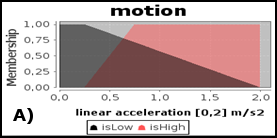
\includegraphics[scale=1.2]{fuzzy-motion.png}
          \end{center}
        }
      \end{frame}
      
      \begin{frame}{Linguistic terms \& membership functions}{Time}
        \pause
        For the time dimension (only once), we define:
        \pause
        \begin{itemize}
          \item the fuzzy linguistic variable \textit{Time};
          \pause
          \item three linguistic terms \textit{Now}, \textit{Recently} and \textit{aWhile};
          \pause
          \item their membership functions $\mu T(t^j_i)$
          \begin{itemize}
            \item degree of membership of the measure timestamp $t^j_i$ in the fuzzy set $T$.
          \end{itemize}
        \end{itemize}
        
        \pause
        \visible<6->{
          \begin{center}
            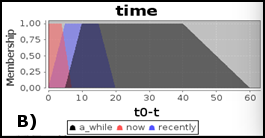
\includegraphics[scale=1.2]{fuzzy-time.png}
          \end{center}
        }
      \end{frame}
      
    \subsection{Intersection membership function}
      \begin{frame}{Intersection membership function}
        \pause
        For each sensor and time linguistic term, we define the intersection membership function:
        \pause
        \begin{itemize}
          \item $V \cap T (m^j_i) = V(v^j_i) \cap T(t^j_i)$
          \begin{itemize}
            \item t-norm $\cap = MIN$;
          \end{itemize}
          \pause
          \item e.g. \textit{High\_motion Recently}.
        \end{itemize}
        
        \pause
        \visible<5->{
          \begin{center}
            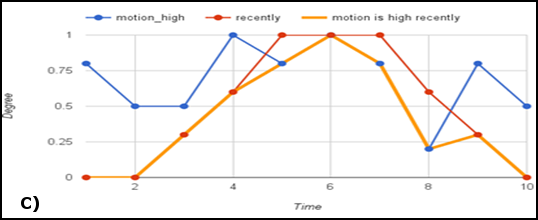
\includegraphics[scale=0.7]{fuzzy-motion_high-recently.png}
          \end{center}
        }
        
        \pause
        The degree of membership of all measures $\{m^j_i\}$ of a sensor $s^j$ to $V \cap T$ is given by aggregation through union:
        \pause
        \begin{itemize}
          \item $V \cap T(s^j) = \bigcup_{m^j_i \in s^j} V \cap T (m^j_i)$
        \end{itemize}
      \end{frame}
      
    \subsection{Rule-based inference engine}
      \begin{frame}{Rule-based inference engine}
        \pause
        A domain expert gives temporal fuzzy rules, through which linguistic terms from multiple sensors can be processed.
        
        \pause
        \vspace{1.5em}
        Fuzzy temporal logic rules have the form:
        \pause
        \begin{center}
          \textit{IF v is V WHEN t is T THEN m IS M}
        \end{center}
        
        \pause
        \vspace{1.5em}
        For example:
        \begin{center}
          \textit{IF (movement IS significant AND inhabitant IS close to living room ) WHEN now AND (inhabitant IS cooking) WHEN a while THEN inhabitant IS eating}
        \end{center}
      \end{frame}
    
  \section{A Stochastic Modelling approach}
    \begin{frame}{Stochastic Models}
      \pause
      \textit{Stochastic Models} represent an approximation of systems where are modelled:
      \pause
      \begin{itemize}
        \item the evolution of the system's state;
        \pause
        \item the stochastic parameters that characterize how the system passes from a state to another.
      \end{itemize}
      \pause
      \visible<5->{
        \begin{center}
          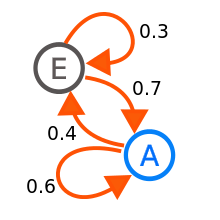
\includegraphics[scale=0.5]{220px-Markovkate_01.png}
        \end{center}
      }
    \end{frame}
    
    \subsection{Process mining}
      \begin{frame}{Process mining}{From annotated datasets to stochastic models}
        \pause
        The term \textbf{process mining} indicates a set of techniques for building a stochastic model of a partially observable system from an annotated dataset of that same system.
        
        \pause
        \vspace{1em}
        Process mining is composed of two main techniques:
        \pause
        \begin{itemize}
          \item \textbf{Process elicitation}: builds the discrete model (i.e., with no information about the sojourn times in different system's state) from events and annotated activities in the dataset.
          \pause
          \item \textbf{Process enhancement}: adds a continuous time vision to the discrete model introducing stochastic parameters that describe how the system evolves during time, using statistical measures calculated from the dataset.
        \end{itemize}
      \end{frame}
      
    \subsection{Possible analyses}
      \begin{frame}{Smart environments analyses}{General schema}
        \vspace{-1em}
        \begin{center}
          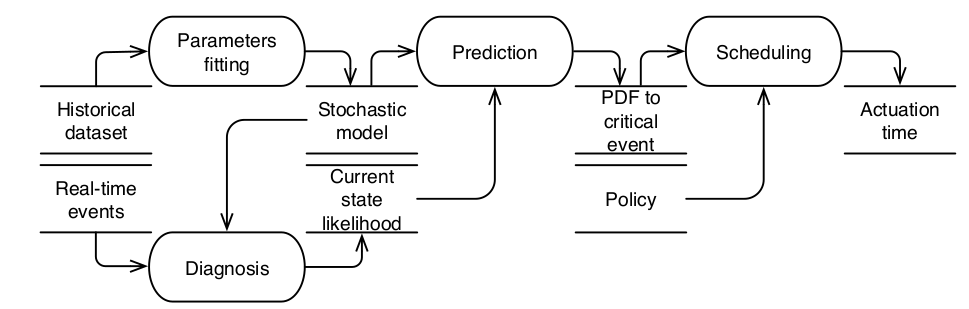
\includegraphics[scale=0.34]{architecture.png}
        \end{center}
        
        \pause
        \begin{itemize}
          \item \textbf{Process mining}: from annotated datasets to stochastic model.
          \pause
          \item \textbf{Diagnosis}: from actual events to likelihood of the current state (on a specific stochastic model).
          \pause
          \item \textbf{Prediction}: from likelihood of the current state to probability that a critical event occurs.
          \pause
          \item \textbf{Scheduling}: from probability that a critical event occurs to time when to schedule the response action (with a specific reaction policy).
        \end{itemize}
      \end{frame}
  
      \begin{frame}{Diagnosis}
      	\begin{center}
      		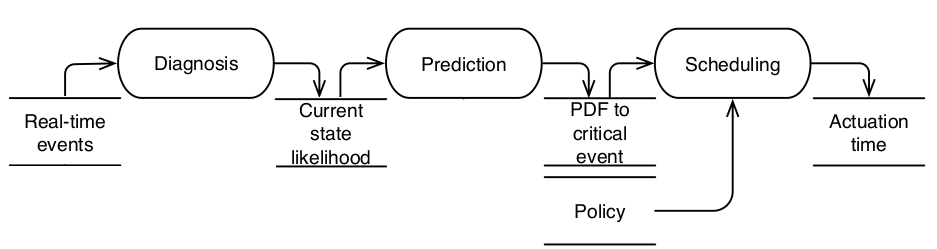
\includegraphics[width=\textwidth,height=0.8\textheight,keepaspectratio]{diag_pred_sched_chain_general.png}
      	\end{center}
      	\begin{tikzpicture}[remember picture, overlay]
        	\node [shift={(-12cm,-5.5cm)}]  at (current page.north east)
        	{%
        		\begin{tikzpicture}[remember picture, overlay]
        			\draw[red, thick] (0,0) rectangle (5cm,2.5cm);
        		\end{tikzpicture}
        	};
      	\end{tikzpicture}
      	
      	\pause
      	\textbf{Diagnosis} computes the most likely actual state of the model at present time, given all the events observed up until the present time.
      \end{frame}
      
    \subsection{H-MRGP-M}
      \begin{frame}{H-MRGP-M}
        \pause
        The \textbf{Hidden-Markov Regenerative Process-Model} (H-MRGP-M) has been developed by STLab at University of Florence.\footnote{Carnevali, L., Nugent, C., Patara, F. and Vicario, E., 2015, September. A continuous-time model-based approach to activity recognition for ambient assisted living. In International Conference on Quantitative Evaluation of Systems (pp. 38-53). Springer International Publishing.}
        
        \pause
        \begin{itemize}
          \item Models the continuous sojourn time in the system's states and the events inter-times.
          \pause
          \item The model's state evolves as a \textit{Markov Regenerative Process} (MRP).
        \end{itemize}
      \end{frame}
      
      \begin{frame}{H-MRGP-M}{Statistical measures}
        \pause
        \begin{itemize}
          \item Experiments on the van Kasteren dataset.
          \pause
          \item Starting from timestamps in the dataset, statistical measures are computed:
          \begin{itemize}
            \item on the sojourn time in each activity;
            \item of the inter-time between events in each activity.
          \end{itemize}
        \end{itemize}
        
        \pause
    		\begin{table}[h!]
    			\centering
    			\small
    			\setlength{\tabcolsep}{5pt}
    			\def\arraystretch{0.75}
    			\begin{tabular}{| l | c | c || c | c |}
    				\hline
    				& \multicolumn{2}{|c||}{\bf Sojourn time}& \multicolumn{2}{|c|}{\bf Inter-time between events}\\
    				\cline{2-5}
    				& $\mu$ (s) & {\bf CV} & $\mu$ (s) & {\bf CV}\\
    				\hline
    				{\bf Leaving house} & 40\,261.455 & 1.042 & 9\,354.190 & 2.810 \\ \hline
    				{\bf Preparing a beverage} &  35.667 & 1.361 & 7.643 & 2.613\\ \hline
    				{\bf Preparing breakfast} &  108.684 & 0.713 & 9.928 & 1.844\\ \hline
    				{\bf Preparing dinner} &  1\,801.889 & 0.640 & 77.966 & 2.589\\ \hline
    				{\bf Sleeping} &  26\,116.571 & 0.442 & 1\,871.836 & 3.090\\ \hline
    				{\bf Taking shower} &  485.910 & 0.298 & 102.788 & 1.969\\ \hline
    				{\bf Toileting} &  88.742 & 1.175 & 14.814 & 2.449\\ 
    				\hline
      		\end{tabular}
    		\end{table}
      \end{frame}
      
      \begin{frame}{H-MRGP-M}{Stochastic model @runtime}
        \pause
        \begin{itemize}
          \item The model is created with \textit{process mining} techniques:
          \pause
          \begin{itemize}
            \item \textit{process elicitation} in order to define the model topology;
            \pause
            \item \textit{process enhancement} in order to add stochastic parameters from the statistical measures calculated (Whitt technique\footnote{Whitt, W., 1982. Approximating a point process by a renewal process, I: Two basic methods. Operations Research, 30(1), pp.125-147.} and software PhFit\footnote{Horváth, A. and Telek, M., 2002, April. Phfit: A general phase-type fitting tool. In International Conference on Modelling Techniques and Tools for Computer Performance Evaluation (pp. 82-91). Springer Berlin Heidelberg.}).
          \end{itemize}
          \pause
          \item Model \textbf{@runtime}: the model is updated each time a new event is observed.\footnote{Blair, G., Bencomo, N. and France, R.B., 2009. Models@ run. time. Computer, 42(10).}
          \pause
          \item The model formalism used is that of \textbf{stochastic Timed Petri Net} (sTPN).\footnote{Horváth, A. and Vicario, E., 2009, September. Aggregated stochastic state classes in quantitative evaluation of non-markovian stochastic Petri nets. In Quantitative Evaluation of Systems, 2009. QEST'09. Sixth International Conference on the (pp. 155-164). IEEE.}\footnote{Vicario, E., 2001. Static analysis and dynamic steering of time-dependent systems. IEEE transactions on software engineering, 27(8), pp.728-748.}
        \end{itemize}
      \end{frame}
      
      \begin{frame}{H-MRGP-M}{sTPN}
        \begin{center}
          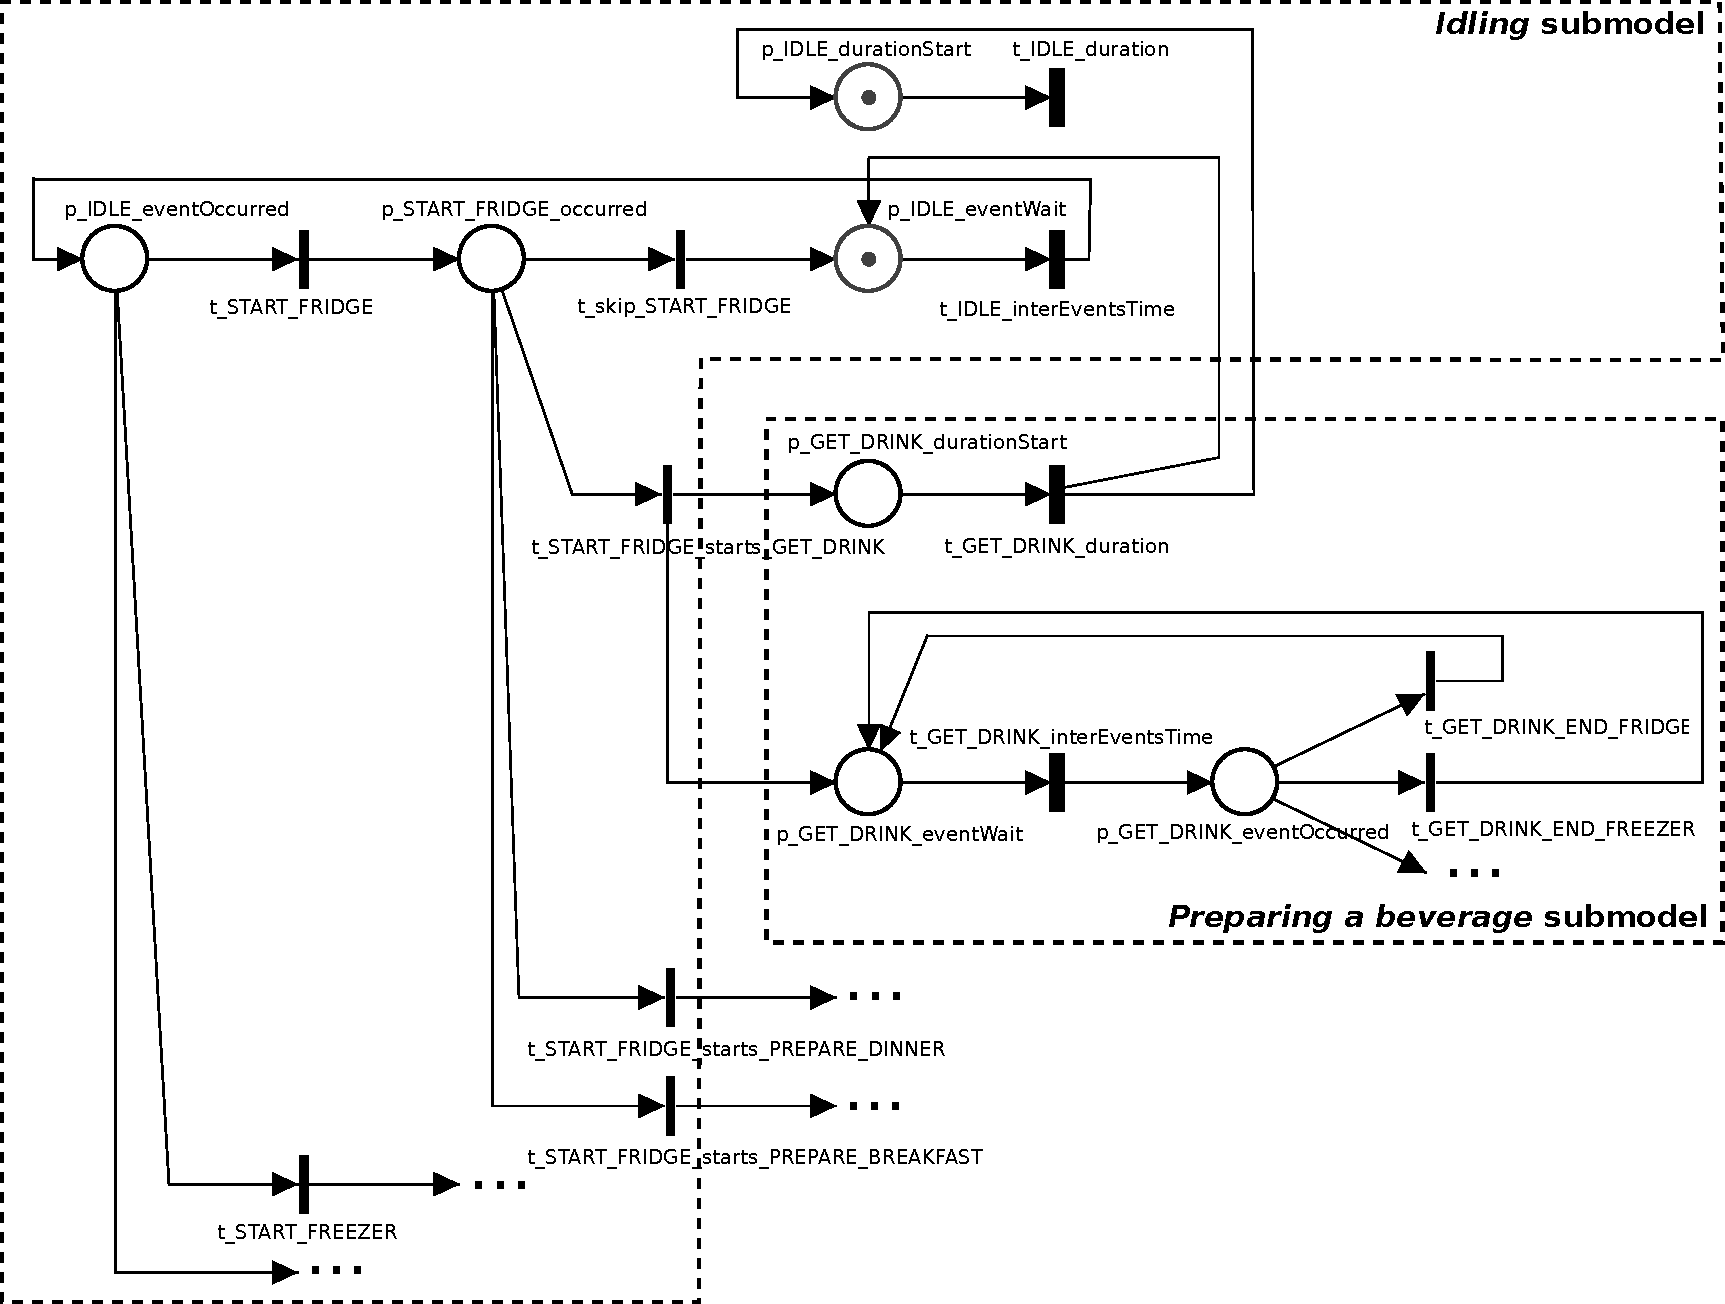
\includegraphics[scale=0.32]{model_withGEN.pdf}
        \end{center}
      \end{frame}
      
      \begin{frame}{H-MRGP-M}{Transient analysis}
        \pause
        After each observation, likelihoods of being in different system's states can be computed up until the next observation.
        \pause
        \begin{itemize}
          \item The transient analysis technique for MRP based on stochastic state classes is exploited.\footnote{Horváth, A., Paolieri, M., Ridi, L. and Vicario, E., 2012. Transient analysis of non-Markovian models using stochastic state classes. Performance Evaluation, 69(7), pp.315-335.}
        \end{itemize}
        
        \pause
        \visible<4->{
          \begin{center}
            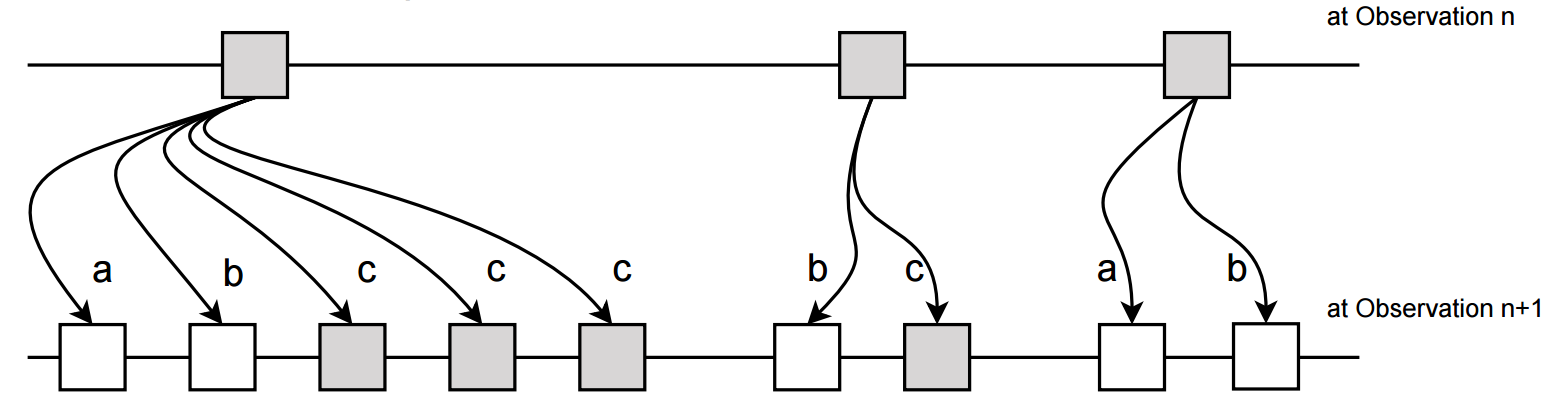
\includegraphics[scale=0.18]{diagnosis-analysis-scheme.png}
          \end{center}
        }
        
        \pause
        The state with highest likelihood is the diagnosed current activity.
      \end{frame}
      
      \begin{frame}{H-MRGP-M}{Transient analysis}
        \begin{center}
          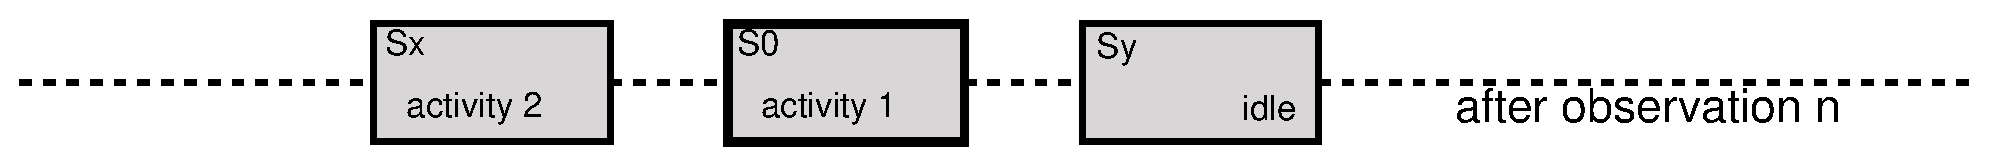
\includegraphics[scale=0.33]{onLineAnalysisAfterN_start.eps}
        \end{center}
        
        \pause
        After having observed the event $n$, for each (possible) current activity
        \pause
        \begin{itemize}
          \item a classes tree is built until the next observation (event $n+1$) is met;
          \pause
          \item leaves corresponding to the new observed event are selected;
          \pause
          \item the PDF of the selected leaves is computed in the delay $d$ (inter-time between events $n$ and $n+1$) in each tree and summing them with weight the root likelihood;
          \pause
          \item the highest is given as most likely current activity.
        \end{itemize}
      \end{frame}
      
      \begin{frame}{H-MRGP-M}{Transient analysis}
        \begin{center}
          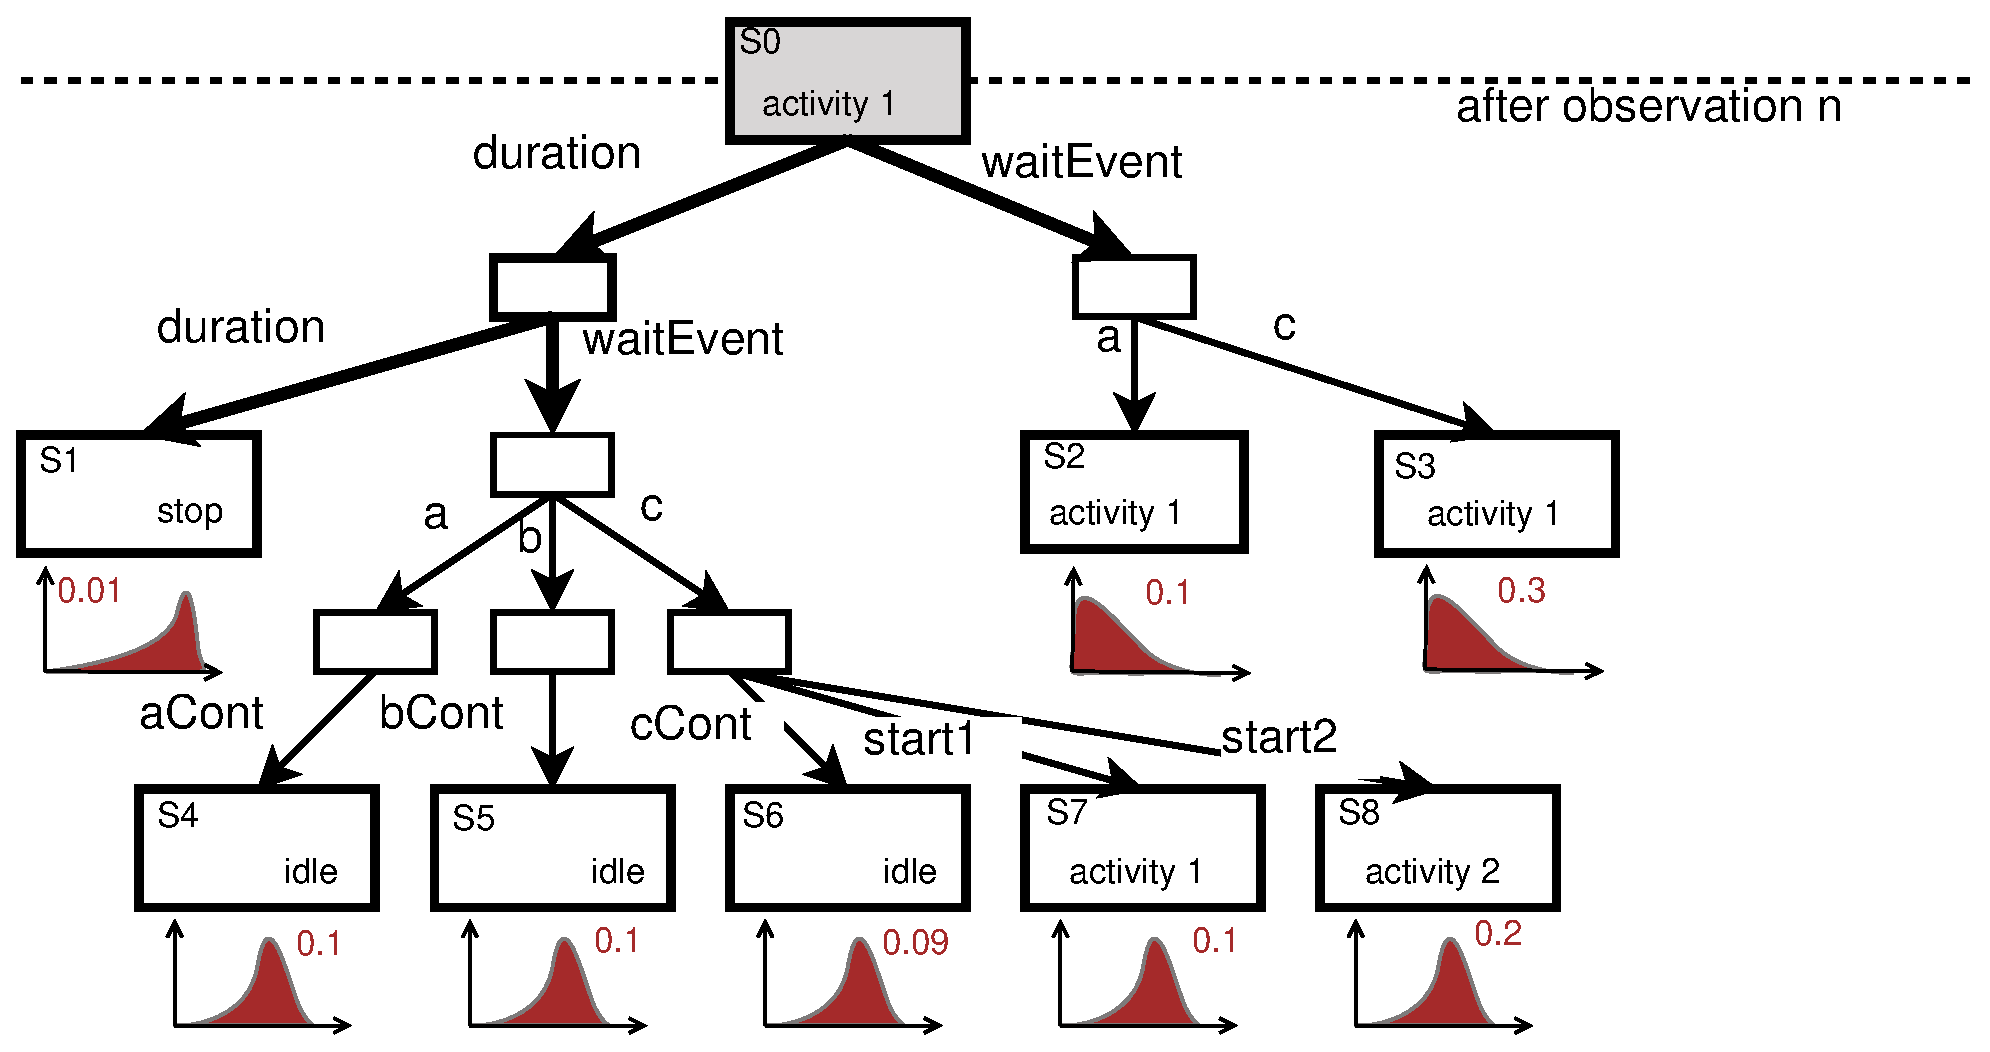
\includegraphics[scale=0.35]{onLineAnalysisAfterN.eps}
        \end{center}
      \end{frame}
      
      \begin{frame}{H-MRGP-M}{Transient analysis}
        \begin{center}
          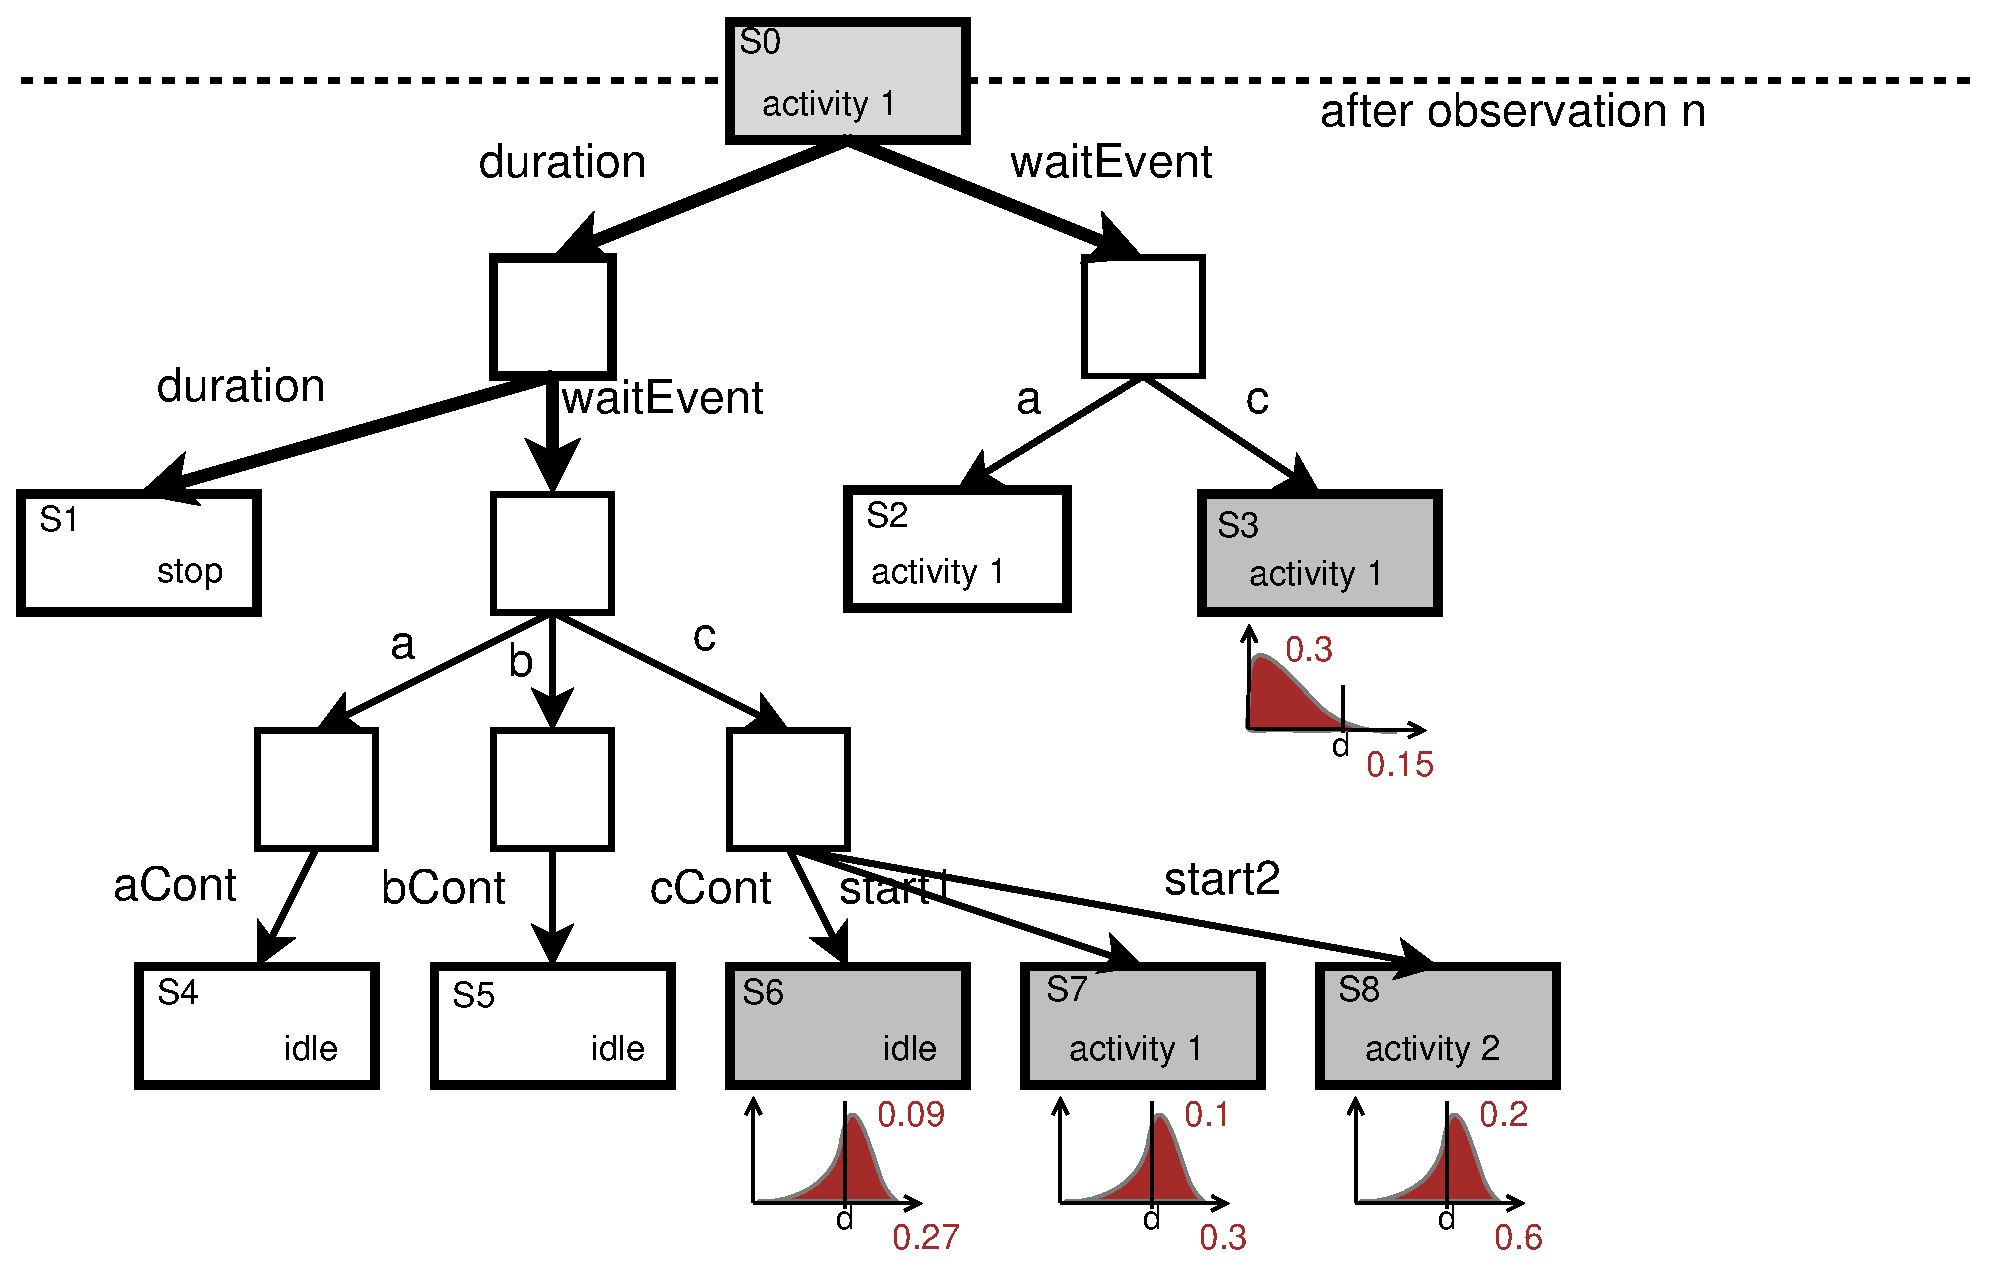
\includegraphics[scale=0.325]{onLineAnalysisAfterN_restricted.eps}
        \end{center}
      \end{frame}
      
  \section{A joint proposal}
    \subsection{Pros \& cons}
      \begin{frame}{Pros \& cons}
        \pause
        The H-MRGP-M model has several pros and cons.\\
        \pause
        \vspace{1em}
        \begin{minipage}{0.4\linewidth}
          Pros:
          \begin{itemize}
            \item DDA;
            \item accurate description of system evolution through stochastic modellization.
          \end{itemize}
        \end{minipage}
        \pause
        \begin{minipage}{0.4\linewidth}
          Cons:
          \begin{itemize}
            \item no support for continuous sensors;
            \item only last event taken into consideration.
          \end{itemize}
        \end{minipage}\\
        \pause
        \vspace{2em}
        Exploiting linguistic terms and temporal fuzzy rules, support for continuous sensors can be added to the H-MRGP-M model!
      \end{frame}
    
    \subsection{Proposals}
      \begin{frame}{Proposal}{Intersection fuzzy set}
        \pause
        \begin{itemize}
          \item Use linguistic variables as before:
          \begin{itemize}
            \item provided by an expert;
            \item one for the time dimension and one for each continuous sensor.
          \end{itemize}
          \pause
          \item Define state-changes for each continuous sensor:
          \begin{itemize}
            \item for each pair of time and sensor-specific linguistic term define the intersection fuzzy set $V \cap T$;
            \item each combination is seen as a different state-change for a specific sensor.
          \end{itemize}
          \pause
          \item The new state-changes of the continuous sensor are added to the model.
        \end{itemize}
        \pause
        When a new continuous event is observed:
        \pause
        \begin{itemize}
          \item compute the degree of membership of the new measurement to the intersection fuzzy sets $V \cap T$;
          \pause
          \item identify the intersection fuzzy set with highest membership degree;
          \pause
          \item the state-change corresponding to the fuzzy set with highest membership degree is fired in the H-MRGP-M model.
        \end{itemize}
      \end{frame}
      
      \begin{frame}{Proposal}{Fuzzy temporal rules}
        \pause
        \begin{itemize}
          \item Use linguistic variables as before:
          \begin{itemize}
            \item provided by an expert;
            \item one for the time dimension and one for each continuous sensor.
          \end{itemize}
          \pause
          \item Define state-changes for each continuous sensor:
          \begin{itemize}
            \item define state-change fuzzy temporal rules (by an expert);
            \item each rule is applied to the whole sensor data stream;
            \item e.g. \textit{IF (movement IS high) WHEN now AND (movement IS low) WHEN a while THEN inhabitant IS started moving}.
          \end{itemize}
          \pause
          \item The new state-changes of the continuous sensor are added to the model.
        \end{itemize}
        \pause
        When a new continuous event is observed:
        \pause
        \begin{itemize}
          \item infer the state-change using the fuzzy temporal rule engine and the sensor data stream;
          \pause
          \item the inferred state-change is fired in the H-MRGP-M model.
        \end{itemize}
      \end{frame}
      
      \begin{frame}{Future proposals}
        \pause
        \begin{itemize}
          \item Full DDA:
          \begin{itemize}
            \item extended belief rule-based inference;\footnote{Espinilla, M., Medina, J., Calzada, A., Liu, J., Martínez, L. and Nugent, C., 2016. Optimizing the configuration of an heterogeneous architecture of sensors for activity recognition, using the extended belief rule-based inference methodology. Microprocessors and Microsystems.}
            \item ANFIS.
          \end{itemize}
          \pause
          \item Sensor-specific time linguistic terms:
          \begin{itemize}
            \item each sensor might have different variation distributions in time;
            \item e.g. a sensor motion might have very rapid and very high variations, while a temperature sensor is usually smoother.
          \end{itemize}
        \end{itemize}
      \end{frame}
      
  \section*{The end}
    \begin{frame}
      \begin{center}
      	\textbf{\calligra\Huge The end.}\\
        
\includegraphics[width=5cm]{ornament.eps}
        
      	\pause
      	\vspace{1cm}
      	{\huge\calligra Questions?\pause{} Thanks!}
      \end{center}
    \end{frame}
      
\end{document}
